\documentclass{article}
\usepackage{amssymb}
\usepackage{amsmath}
\usepackage{graphicx}
\newtheorem{theorem}{Theorem}[section]
\newtheorem{corollary}{Corollary}[theorem]
\newtheorem{lemma}{Lemma}[theorem]
\newtheorem{identity}{Identity}[theorem]
\newtheorem{definition}{Definition}[section]
\newcommand{\qed}{\rule{0.7em}{0.7em}}
\begin{document}
\title{Elementi di analisi reale}
\maketitle
\section{L'insieme dei numeri reali: $\mathbb{R}$}
    $\mathbb{R}$ è un:
    \begin{itemize}
        \item \textbf{campo}: rimando alla definizione di campo a fine appunti
        \item \textbf{ordinato}: presenta una relazione d'ordine totale $\leq$
        \item \textbf{completo}: $\forall S \subset \mathbb{R} \textrm{ t.c. } S 
            \textrm{ superiormente limitato } \exists\sup\left(S\right) \in \mathbb{R}$
    \end{itemize}
    Quest'ultima proprietà è detta \textbf{assioma di completezza}, ed è equivalente 
    all'assioma di separazione. \\
    Possiamo notare come la completezza di $\mathbb{R}$ non debba essere collegata al 
    fatto che $\mathbb{R}$ sia ordinato. Pensiamo infatti a $\mathbb{C}$, insieme non 
    ordinato ma che, essendo isomorfo a $\mathbb{R}^2$, dovrà essere necessariamente completo.
    \subsection{Successioni in $\mathbb{R}$}
        \begin{definition}[Successione]
            \, \\ Una successione in $\mathbb{R}$ è una funzione 
            $$f\left(n\right): \mathbb{N} \to \mathbb{R}$$
        \end{definition}
        Si dice che per una successione $\{a_n\}$ vale una certa proprietà $P\left(n\right)$
        \begin{itemize}
            \item \textbf{definitivamente} se $\exists N \in \mathbb{N} \textrm{ t.c. } \forall n \geq N$ vale $P\left(n\right)$
            \item \textbf{frequentemente} se $\forall m \in \mathbb{N} \, \exists n \in \mathbb{N} \textrm{ t.c. } n \geq m$ vale $P\left(N\right)$
        \end{itemize}
        Una successione $\{a_n\}$ è detta:
        \begin{itemize}
            \item \textbf{limitata} se $\forall n \in \mathbb{B}, \exists a, b \in \mathbb{R} \textrm{ t.c. } a \leq a_n \leq b$. Se ciò vale
                solo per un estremo è detta limitata dall'alto/basso
            \item \textbf{monotona} crescente/decrescente se $\forall n \in \mathbb{B}, a_n \leq/\geq a_{n+1}$
            \item \textbf{convergente} in un insieme ${X}$ se $\exists l \in X \land \forall \varepsilon > 0 |a_n - l| < \varepsilon$ definitivamente
            \item \textbf{divergente} a $\pm \infty$ se $\forall M > 0, a_n >/< \pm M$ definitivamente 
            \item \textbf{non convergente} in un insieme $X$ se non converge in $X$ e non diverge
        \end{itemize}
        Infine, data $\{a_n\}$ sono detti:
        \begin{itemize}
            \item limite superiore della successione ($\lim_{n \to \infty} \sup \{a_n\}$): il minor maggiorante della successione per $n \to \infty$
            \item limite inferiore della successione ($\lim_{n \to \infty} \inf \{a_n\}$): il maggior minorante della successione per $n \to \infty$
        \end{itemize}
        Prendendo spunto dalle funzioni, possono essere pensati come una coppia di \textit{"quasi-asintoti"} che limitano la successione.
        \begin{center}
            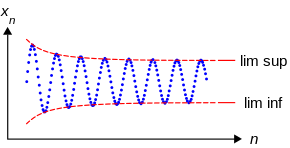
\includegraphics{limsupinf.png}
        \end{center}
        \begin{definition}[sottosuccessione] \, \\
            Una successione $\{a^*_n\} \subset \{a_n\}$ è detta sottosuccessione se esiste una funzione 
            $$\varphi\left(n\right): \mathbb{N} \to \mathbb{N} \textrm{ strettamente crescente t.c. } a^*_k = a_{\varphi\left(k\right)}$$
        \end{definition}
        \begin{theorem}[Teorema di Bolzano-Weistrass]
            $$\forall \{a_n\} \textrm{ limitata } \exists\{a^*_n\} \subset \{a_n\} \textrm{ convergente }$$
        \end{theorem}
        \textit{Dimostrazione}: \\
            Costruiamo un insieme $I$ di indici dei\textit{"picchi"} della successione $\{a_n\}$ ovvero 
            $$I = \{i: a_i \geq a_{i+n} \forall n \in \mathbb{N}\}$$
            Abbiamo ora due opzioni:
            \begin{itemize}
                \item $|I| = \infty$: ne consegue che la sottosuccessione $\{a_i\}_{i \in I}$ è monotona decrescente e quindi convergente
                \item $|I| \in \mathbb{N}$: $\exists N \in \mathbb{N} \textrm{ t.c. } \forall i \in I, i < N \implies$ \\
                    $|M = \{m: \forall n > N m > n \land a_m \leq a_n\}| = \infty \implies \{a_m\}_{m \in M}$ monotona crescente e quindi convergente $\; \qed$
            \end{itemize}
        Questa dimostrazione fa uso dell'assioma di completezza assumendo che una successione limitata abbia l'estremo superiore ed inferiore.
        \begin{definition}[Successione di Cauchy]
            $$\{a_n\} \textrm{ è detta di Cauchy se } \forall \varepsilon > 0, \forall m > n |a_n - a_m| < \varepsilon \textrm{ definitivamente }$$
        \end{definition}
        \begin{theorem}[Una successione convergente è di Cauchy]
            $$\{a_n\} \textrm{ convergente } \implies \{a_n\} \textrm{ di Cauchy }$$
        \end{theorem}
        \textit{Dimostrazione}: \\
        $$\{a_n\} \to l \implies \exists N \in \mathbb{N} \textrm{ t.c. } \forall n > N |a_n - l| < \varepsilon \implies $$
        $$ \forall m > n, |a_n - l| + |l - a_m| < 2\varepsilon \implies |a_n - a_m| < 2\varepsilon \; \qed$$
        \begin{theorem}[Convergenza delle successioni di Cauchy]
            $$\{a_n\} \textrm{ di Cauchy } \implies \{a_n\} \textrm{ convergente }$$
        \end{theorem}
        \textit{Dimostrazione}:\\
        $$\{a_n\} \textrm{ di Cauchy } \implies \exists K \in \mathbb{N} \textrm{ t.c. } \forall m, n > K |a_m - a_n| < \varepsilon_0 \implies a_n - \varepsilon_0 < a_m < a_n + \varepsilon_0$$
        Consideriamo ora $S_n = \min\{a_i \forall i < n\} \cup \{a_n - \varepsilon_0, a_n + \varepsilon_0\}$, ne deriva che
        $$\forall m \in \mathbb{N}, \min S_n < a_m < \max S_n \implies \{a_n\} \textrm{ limitata}$$
        Per Bolzano-Weistrass ne consegue che esiste una sottosuccessione $\{a_{\varphi_i}\}$ convergente a $l$, ovvero 
        $$\exists M \in \mathbb{N} \textrm{ t.c. } \forall \varphi_i \geq M |a_{\varphi_i} - l| < \varepsilon_1$$ 
        Ne consegue che
        $$\forall n, i \in \mathbb{N} \textrm{ t.c } n, \varphi_i >  \max\left(K, M\right),
            |a_n - a_{\varphi_i}| + |a_{\varphi_i} - p| < \varepsilon_0 + \varepsilon_1 \implies |a_n - p| < \varepsilon_0 + \varepsilon_1 \; \qed$$  
        Risulta ovvio come, in quanto Bolzano-Weistrass richiede l'AoC, anche questa dimostrazione richieda l'AoC
        \subsection{Dimostrazione dell'AoC}
            L'assioma di completezza è un assioma \textit{"forte"}, ed è quindi preferibile che si potesse in qualche modo 
            derivare, che è quello che ora faremo. Introduciamo prima una proprietà molto importante
            \begin{theorem}[Proprietà archimedea]
                $$\forall x \in \mathbb{R}, \exists n \in \mathbb{N} \textrm{ t.c. } x < n$$
            \end{theorem}
            \begin{corollary}[Convergenza di $\frac{1}{n}$ a $0$]
                $$\forall x \in \mathbb{R}, \exists n \in \mathbb{N} \textrm{ t.c. } \frac{1}{n} < x$$
            \end{corollary}
            \begin{corollary}[Densità di $\mathbb{Q} \in \mathbb{R}$]
                $$\forall a, b \in \mathbb{R}, \exists q \in \mathbb{Q} \textrm{ t.c. } a < q < b$$
            \end{corollary}
            Tutte è tre le dimostrazioni sono abbastanza semplici e lasciate al lettore (in più, come esercizio, 
            dimostrare che $\forall a, b \in \mathbb{Q}, \exists r \in \mathbb{R} - \mathbb{Q} \textrm{ t.c. } a < r < b$). \\
            Procediamo ora col nostro obbiettivo
            \begin{theorem}[Assioma di completezza] 
                $$\{a_n\} \textrm{ di Cauchy } \implies \{a_n\} \textrm{ converge } \implies \textrm{AoC}$$
            \end{theorem}
            \textit{Dimostrazione}:
            $$E \subset \mathbb{R}, E \textrm{ superiormente limitato } \implies \exists b_0 \textrm{ maggiorante di } E$$
            Costruiamo ora due successioni $\{a_n\}, \{b_n\}$ così costruite:
            \begin{enumerate}
                \item Scegliamo $a_0 \in E$
                \item Consideriamo $k = \frac{a_n + b_n}{2}$
                \item Se $k \in E$, $a_{n+1} = k, b_{n+1} = b_n$, in alternativa $a_{n+1} = a_n, b_{n+1} = k$
            \end{enumerate}
            Facile notare come $\forall n, b_{n+1} - a_{n+1} = \frac{b_n - a_n}{2}$, il che implica che 
            $$\forall n, |a_n - b_n| = \frac{b_0 - a_0}{2^n}$$
            Ciò implica che $\{a_n\},\{b_n\}$ sono di Cauchy in quanto 
            $$|a_{n+j} - a_n| < b_n - a_n \land |b_{n+j} - b_n| < b_n - a_n \; \forall j \in \mathbb{N}$$
            In quanto per la proprietà archimedea $\frac{b_0 - a_0}{2^n} \to 0$, allora anche $b_n - a_n \to 0$, il che 
            verifica che le nostre due successioni sono di Cauchy. \\
            Inoltre per $n \to \infty$, $a_n = b_n$, ed essendo di Cauchy ne deriva che convergono entrambe a limite $l$, che 
            per costruzione è maggiorante di $E$. \\
            Ipotizziamo ora che esista $p$ maggiorante di 
            $E$ tale che $p < l$. Ne seguirebbe che, $\forall n \in \mathbb{N}, p > l$ per costruzione, e quindi 
            abbiamo $\forall n, a_n < p < l$. Passando al limite, otteniamo che $l < p < l$ il che è impossibile, 
            e quindi $l$ è il minor minorante di $E$, dimostrando l'AoC $\; \qed$
        \subsection{Considerazioni importanti}
            I più attenti avranno notato che ad inizio capitolo abbiamo parlato di come vogliamo 
            rendere separati i concetti di completezza e di ordinamento di un insieme, ma che 
            questo il concetto di ordinamento è usato nella definizione stessa delle successioni di 
            Cauchy, ed è quindi usato nella nostra dimostrazione dell'AoC. \\
            Si propone di sostituire il concetto di ordinamento col concetto di \textbf{distanza}, che 
            verrà introdotto nel prossimo capitolo 
\newpage
\section{Spazi metrici}
\end{document}